%%
%% GPW2026 Extended Abstract (下書き) -- ゲームプログラミングワークショップ
%% ベース: gi58/draft.tex (IPSJ SIG-GI58) のスタイルを流用。
%% 制約: A4縦, 2段組, 10pt以上, PDF 2ページ以内。
%%
%% TODO (要更新): 下の \newcommand 群は速報値(seed42のみ)。
%%   bearでのA1d1 5シード分完走後、scripts/analyze_cluster_switch.py と
%%   scripts/analyze_a9_validity.py を再実行し、数値を差し替えること。
%%   差し替え箇所はこの \newcommand 定義だけでよい設計にしてある。
%%

\documentclass[submit,techrep,noauthor]{ipsj}

\usepackage{graphicx}
\usepackage{latexsym}
\usepackage{amsmath,amssymb}
\usepackage{url}

\def\Underline{\setbox0\hbox\bgroup\let\\\endUnderline}
\def\endUnderline{\vphantom{y}\egroup\smash{\underline{\box0}}\\}
\def\|{\verb|}

%% ===== 数値プレースホルダ (要・実験完了後の更新) =====
% run50v2 regret (P=200, 5seed, 修正木, commit ebb5f80)
\newcommand{\regretAone}{0.514}
\newcommand{\regretAtwo}{0.506}
\newcommand{\regretAfive}{0.505}
\newcommand{\regretAseven}{0.502}
\newcommand{\regretAeight}{0.511}
\newcommand{\regretAnine}{0.508}
\newcommand{\friedmanP}{0.88}
% A9 vs A2 head-to-head (run50v2)
\newcommand{\aNineVsAtwoDq}{-0.002}
% A9 クラスタ価値の妥当性 (5seed, commit f0cb2f6)
\newcommand{\rhoCluster}{0.49}
\newcommand{\rhoCandidate}{0.30}
% クラスタ乗り換え分析 (現状 seed42速報値、要5seed化)
\newcommand{\switchEndgame}{55\%}
\newcommand{\switchMidgame}{90\%}
\newcommand{\switchOpening}{100\%}
\newcommand{\agreeEndgame}{31\%}
\newcommand{\agreeMidgame}{9\%}
\newcommand{\agreeOpening}{7\%}

\begin{document}

\title{デジタルカーリングにおけるMCTS候補手削減のための\\価値考慮型クラスタリングとその分析的応用}

\etitle{Value-Aware Clustering for Action Space Reduction \\ and Its Analytical Use in MCTS for Digital Curling}

\affiliate{MU}{明治大学\\
Meiji University}

\author{仲 亜斗夢}{Atomu Naka}{MU}[ce265004@meiji.ac.jp]
\author{横山 大作}{Daisaku Yokoyama}{MU}[dyokoyama@meiji.ac.jp]

\begin{abstract}
デジタルカーリングにおけるモンテカルロ木探索(MCTS)では，連続な行動空間から生成した多数の候補手を，結果盤面の類似性に基づく階層的クラスタリングにより削減する手法(Proposed)が既に提案されている．
しかし，Proposedは各クラスタの代表手を盤面的な中心性(medoid)のみで選出しており，得点の観点で有望な手を取りこぼす可能性があった．
本研究では，各候補の得点期待値を安価に推定し，クラスタの平均得点期待値に基づいて代表手を選出する手法(ClusterValue)を提案する．
等予算下での評価実験の結果，提案手法は全探索および従来手法(Proposed)と同等の意思決定品質を，性能を犠牲にすることなく維持できることを確認した．
さらに，クラスタ単位の得点期待値は審判値($K{=}200$回のリサンプリングによる推定得点)と有意な相関(候補単位$\rho\fallingdotseq\rhoCandidate$に対しクラスタ単位$\rho\fallingdotseq\rhoCluster$)を示し，盤面上の戦略的に有望なエリアを可視化する分析基盤として機能することを示した．
加えて，探索深さを変えた際に選ぶ手が変化する現象を，このクラスタ構造を用いて分析した結果，終盤では変化の多くがクラスタ(戦術)単位の乗り換えであることが明らかになった．
\end{abstract}

\maketitle

%% ======================================================================
\section{はじめに}

デジタルカーリング\cite{dc3}は，連続行動空間と実行時ノイズによる確率的不確定性を併せ持つ戦略ゲームであり，MCTSを用いた候補手選択には計算コストの課題がある．
先行研究\cite{owatari2016,kato2016}やわれわれの既報\cite{naka_gi58}では，候補手生成後の結果盤面に対して階層的クラスタリングを適用し，各クラスタの代表手のみをMCTSの子ノードとして残すことで探索対象を削減する手法(以下Proposed)を検討してきた．

しかし，Proposedの代表手選出は各クラスタ内で盤面的に最も中心的な候補(medoid)を機械的に選ぶのみであり，得点の観点からの手の良し悪しを一切考慮していない．
このため，同一クラスタ内に得点期待値の高い候補と低い候補が混在する場合，代表手が必ずしも有望な手にならないという課題があった．
実際に，等予算下でのregret評価(選んだ手と真の最良手との得点期待値差)において，Proposedはクラスタリングを行わずランダムに候補を間引く手法と有意差がなく，クラスタリングによる寄与が確認できなかった．

本研究では，この課題に対し，クラスタの表現(結果盤面の類似性)は維持したまま，代表手の選出規則にのみ得点期待値を組み込む手法ClusterValueを提案する．
これにより，(i) Proposedの意思決定品質上の弱点を性能低下なく補いつつ，(ii) クラスタという単位が持つ「盤面の戦略的な区分け」としての解釈可能性を活かし，探索対象の可視化・分析基盤として発展させることを目指す．

%% ======================================================================
\section{提案手法: ClusterValue}

ClusterValueは，MCTSのルートノードにおいて以下の手順で候補手を選別する．
(1) 各候補手について，安価なロールアウト(既定3回)により得点期待値$\hat{E}[\mathrm{score}]$を推定する．
(2) Proposedと同一の距離関数・階層的クラスタリング(平均連結法)により，結果盤面を基準に候補手をクラスタへ分割する．
(3) 各クラスタの価値を，メンバー候補の$\hat{E}[\mathrm{score}]$の平均値として定義する．クラスタ単位で平均を取ることで，個々の候補の推定に含まれる分散を低減できる．
(4) 価値上位$K$個のクラスタを採用し，各クラスタ内で$\hat{E}[\mathrm{score}]$が最大の候補を代表手としてMCTSの子ノードに割り当てる．全体の最良候補が属するクラスタは，価値順位によらず必ず採用する．

Proposedとの差異は(3)(4)のみであり，探索木の構造・ロールアウト方策・木の深さ以降の展開は共通である．
したがって両手法の比較は，「代表手選出規則を盤面中心性から得点期待値ベースへ変更した効果」を単離して評価できる．

%% ======================================================================
\section{実験と結果}

\subsection{実験設定}
自己対戦から抽出した50局面$\times$5乱数系列に対し，AllGrid(全候補を子ノードとする基準手法，以下A1)，Proposed(A2)，ランダム間引き(A5)，ClusterValue(A9，提案手法)を含む複数手法を等物理シミュレーション予算下で評価した．
真の最良手の推定には，各候補を実行ノイズ込みで$K{=}200$回再試行する審判機構を別途構築し，regret(審判の最良値との差)を評価指標とした．

\subsection{意思決定品質: 性能を犠牲にしない}
5手法のregretは A1: \regretAone，A2: \regretAtwo，A5: \regretAfive，A7(得点スクリーン型\cite{naka_gi58}): \regretAseven，A8: \regretAeight，\textbf{A9: \regretAnine} であり，Friedman検定でも有意差は見られなかった($p={\friedmanP}$)．
特にA9とA2の局面対応比較では差はほぼ0(\,$\Delta q = \aNineVsAtwoDq$\,)であり，\textbf{代表手選出を得点期待値ベースに変更しても意思決定品質は損なわれない}ことが確認された．
これは，性能の善し悪しではなく，クラスタという表現の上に安全に価値情報を載せられることを意味する．

\subsection{クラスタ価値の妥当性とエリア価値マップ}
クラスタ価値$\hat{E}[\mathrm{score}]$の平均が審判値をどの程度言い当てているかを，5乱数系列すべてでSpearman順位相関により検証した．
候補単位の相関は中央値$\rho\fallingdotseq\rhoCandidate$であるのに対し，クラスタ単位の相関は中央値$\rho\fallingdotseq\rhoCluster$であり，\textbf{5系列すべてで}クラスタ単位の方が高い精度を示した．
これは(3)で述べた分散低減の効果が実データで裏付けられたことを意味する．

\begin{figure}[tb]
\centering
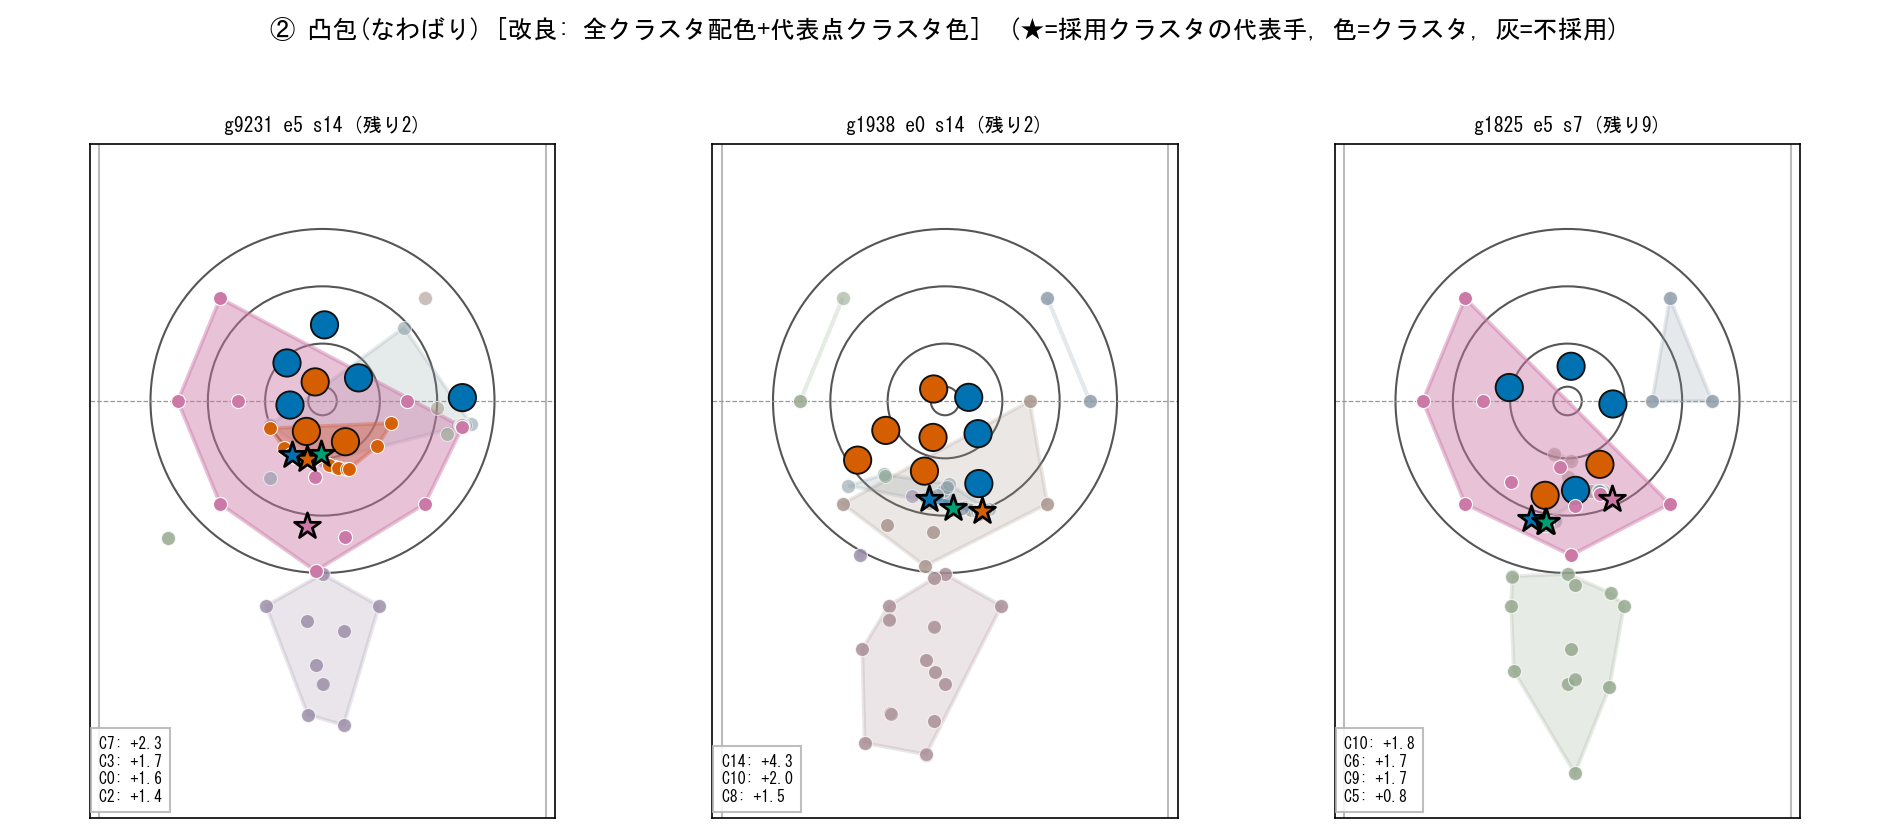
\includegraphics[width=\columnwidth]{figures/area_map_B_hull_draft.png}
\caption{エリア価値マップの例．採用クラスタを色分けした凸包で表示し(灰色は不採用クラスタ)，星印は各クラスタの代表手，数値はクラスタの得点期待値．どのエリアへの投球が有望かを可視化できる．}
\label{fig:areamap}
\end{figure}

この性質を用いて，図\ref{fig:areamap}のように，盤面上のどのエリア(戦術グループ)が得点的に有望かを可視化する「エリア価値マップ」を構成できる．
Proposedの代表手は盤面的な中心性のみで選ばれるため意味付けができなかったが，ClusterValueでは各クラスタに定量的な価値ラベルを付与できるため，局面ごとの戦略的な見取り図として利用できる．

\subsection{探索深さとクラスタ構造の関係}
探索の深さを変えるとMCTSが選ぶ手がどう変化するかを，クラスタ構造を通じて分析した．
深さ3(d3)と深さ1(d1)で選択が一致する割合は，残り手数が少ない終盤ほど低下する(序盤\agreeOpening，中盤\agreeMidgame，終盤\agreeEndgame; 残り手数で3区分)．
選択が分かれた場合に，それが同一クラスタ内の微調整か，別クラスタ(戦術)への乗り換えかを調べたところ，乗り換えの割合は終盤\switchEndgame，中盤\switchMidgame，序盤\switchOpening であった．
さらに終盤で乗り換えが生じたクラスタは常に複数候補を含んでおり(単独候補への収束ではない)，深さの変化が個々の候補ではなく戦術グループ単位の再考を引き起こしていることが示唆される．

\begin{figure}[tb]
\centering
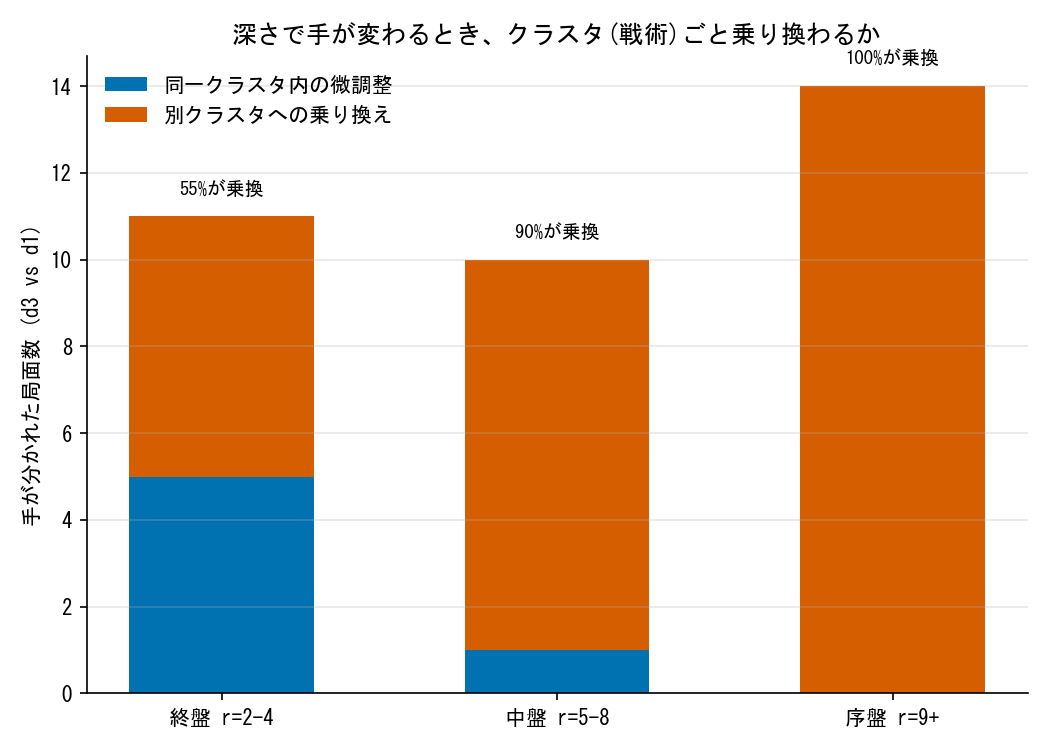
\includegraphics[width=\columnwidth]{figures/cluster_switch_draft_seed42.png}
\caption{深さで手が変わる際の，クラスタ単位での乗り換え割合(残り手数の区分別，速報値)．}
\label{fig:switch}
\end{figure}

%% ======================================================================
\section{おわりに}

本研究では，Proposedのクラスタ表現を維持したまま代表手選出のみを得点期待値ベースに改めるClusterValueを提案した．
提案手法は既存手法と同等の意思決定品質を維持しつつ，クラスタ単位の得点期待値推定が実際の得点期待値と有意に相関することを確認し，盤面の戦略的なエリアを可視化する分析基盤としての価値を示した．
また，この枠組みを用いることで，探索深さによる手の変化がクラスタ(戦術)単位の乗り換えとして観察できることを明らかにした．
今後は，クラスタ価値へのリスク(実行時ノイズ)情報の統合，および終盤の乗り換え現象を踏まえた深さ・予算の動的配分による効率化を検討する．

\begin{thebibliography}{10}

\bibitem{owatari2016}
大渡勝己，田中哲朗：
モンテカルロ木探索によるデジタルカーリングAI，
第21回ゲームプログラミングワークショップ, pp. 180--187 (2016).

\bibitem{kato2016}
加藤修，飯塚博幸, 山本雅人：
不確定性を含むデジタルカーリングにおけるゲーム木探索，
情報処理学会論文誌，Vol.2016-GI-57, No.11, pp.~2354--2364 (2016).

\bibitem{dc3}
北清勇磨，岡田雷太，伊藤毅志：
デジタルカーリングサーバーの提案と紹介，
情報処理学会研究報告. GI, [ゲーム情報学] 2014(2)，pp.~1--5 (2014).

\bibitem{naka_gi58}
仲 亜斗夢，横山 大作：
デジタルカーリングにおけるMCTS候補手削減のためのクラスタリング適用の試み，
情報処理学会研究報告. GI, [ゲーム情報学] 2026-GI-58 (2026).

\end{thebibliography}

\end{document}
